% ==============================================================================
% DASK 2026 - Yarışma Soruları
% İstanbul Finans Merkezi (41.002136°, 29.106832°)
% ==============================================================================
\documentclass[12pt,a4paper]{article}
\usepackage[utf8]{inputenc}
\usepackage[T1]{fontenc}
\usepackage{lmodern}
\usepackage[shorthands=off,turkish]{babel}
\usepackage{geometry}
\usepackage{graphicx}
\usepackage{pgfplots}
\usepackage{booktabs}
\usepackage{amsmath}
\usepackage{tikz}
\usetikzlibrary{shapes.geometric, positioning, arrows.meta}
\usepackage{float}
\usepackage{hyperref}
\usepackage{fancyhdr}
\usepackage{lastpage}
\usepackage{amssymb}
\usepackage{textcomp}

% Güzel Roman rakamları için makro (Türkçe babel uyumlu)
\makeatletter
\newcommand{\RN}[1]{\@Roman{#1}}
\makeatother

\geometry{margin=2.5cm, headheight=14.5pt}
\pgfplotsset{compat=1.17}
\setlength{\parindent}{1.5em}

\hypersetup{
    colorlinks=true,
    linkcolor=blue,
    citecolor=blue,
    urlcolor=blue
}

% Header/Footer
\pagestyle{fancy}
\fancyhf{}
\fancyhead[L]{DASK 2026}
\fancyhead[R]{İstanbul Finans Merkezi Proje Teklifi}
\fancyfoot[C]{\thepage/\pageref{LastPage}}
\renewcommand{\headrulewidth}{0.4pt}
\renewcommand{\footrulewidth}{0.4pt}

\begin{document}

% ==============================================================================
% SORU 1
% ==============================================================================
\section{Sorular}
\subsection{Soru \RN{1}}

\textbf{Soru:} Yapı taşıyıcı sistemini belirlerken nelere dikkat ettiğinizi depreme dayanıklı bina tasarım ilkeleri çerçevesinde (taşıyıcı elemanların geometrisi ve yerleşimi, yeterli dayanım, rijitlik ve sünekliğin sağlanması gibi) açıklayınız.

\textbf{Cevap:} Taşıyıcı sistem seçiminde beş temel ilkeye dikkat edilmiştir: (1)~simetri ve düzenlilik, (2)~yeterli rijitlik, (3)~sürekli yük aktarımı, (4)~süneklik, (5)~hafiflik. TBDY 2018 ve uluslararası tasarım esasları çerçevesinde bu ilkeler aşağıda açıklanmıştır~\cite{tbdy2018, nehrp2009}.

\subsubsection{İkiz Kule ve Köprü Sistemi \& Simetri ve Düzenlilik}

Yüksek katlı yapı konfigürasyonu olarak iki ayrı kule ve bunları birbirine bağlayan köprü elemanlarından oluşan bir sistem tasarlanmıştır. Her kule 26 kattan oluşmakta olup $8 \times 4$ kolon gridi üzerine inşa edilmiştir. Literatürdeki çalışmalar, köprü bağlantılarının yapı yüksekliğinin $1/4$, $1/2$ ve $3/4$ seviyelerine yerleştirilmesinin sismik performansı optimize ettiğini göstermektedir~\cite{patoliya2023}. Bu doğrultuda köprüler yaklaşık olarak 6., 12., 18. ve 25. katlara konumlandırılmıştır. Bu konfigürasyon, yatay yükler altında kulelerin birlikte çalışmasını sağlamakta ve tek bir yüksek kuleye kıyasla daha dengeli yük dağılımı sunmaktadır. Yapının planda ve düşeyde düzenli olması, burulma düzensizliğini önlemek açısından temel gerekliliktir. İkiz kule sistemi her iki ana eksende ($X$, $Y$) simetrik olarak tasarlanmış; kütle merkezi ile rijitlik merkezi arasındaki eksantrisite en aza indirilmiştir. A1a burulma düzensizliği katsayısı $\eta_{bi} = 1.112 < 1.4$ koşulunu sağlamakta olup yapı düzenli sınıfındadır~\cite{teblig2024}.

\subsubsection{Yeterli Yanal Rijitlik \& Sürekli Yük Aktarımı ve Süneklik}

Deprem yüklerinin güvenle temele aktarılması için yapının yatay kuvvetlere karşı yeterli rijitliğe sahip olması gerekmektedir. Çerçeve-çapraz hibrit sistem tercih edilerek, moment taşıyan çerçevelerin sünekliği ile çapraz elemanların rijitliği bir arada kullanılmıştır. Çapraz elemanlar $XZ$ ve $YZ$ düzlemlerinde stratejik noktalara yerleştirilmiş; köprü bağlantısı ise iki kule arasında yük paylaşımını sağlayarak global sistem rijitliğini artırmıştır. Deprem yüklerinin kesintisiz olarak temele iletilmesi için düşey taşıyıcı elemanlar tüm katlarda aynı konumda devam etmektedir. Kolon-kiriş düğüm noktaları rijit bağlantılı, çapraz elemanlar mafsallı modellenmiştir. Güçlü kolon--zayıf kiriş tasarım prensibi uygulanarak plastik mafsalların kiriş uçlarında oluşması hedeflenmiştir. CQC yöntemiyle hesaplanan göreli kat ötelemesi $\delta/h = 0.00117 < 0.008$'dir~\cite{tbdy2018}.

\subsubsection{Hafiflik ve Malzeme}

Deprem kuvvetleri yapı kütlesi ile doğru orantılı olduğundan, taşıyıcı sistemin mümkün olduğunca hafif tutulması esastır. Balsa ahşap malzeme ($E = 3.5$~GPa) kullanılarak yapısal analizler \textsc{OpenSees}\textsuperscript{\textregistered} yazılımı ile gerçekleştirilmiş~\cite{opensees}, ağırlık minimizasyonu ve rijitlik maksimizasyonu hedefleriyle iteratif optimizasyon yapılmıştır. \href{https://github.com/adzetto/DASK_26__DESIGN_AND_ANALYSIS}{\textcolor{blue}{Github deposunda}} tüm analiz ve optimizasyon kodları mevcuttur~\cite{github_repo}.

Sonuç olarak, sahaya özgü deprem tehlikesi parametreleri ($S_{DS} = 1.008$~g, $S_{D1} = 0.514$~g, zemin sınıfı ZD) dikkate alınarak~\cite{afad2024}, TBDY 2018 gerekliliklerini karşılayan simetrik, rijit, sünek ve hafif bir ikiz kule--köprü taşıyıcı sistem tasarlanmıştır.

\newpage

% ==============================================================================
% SORU 2 (Placeholder)
% ==============================================================================
\subsection{Soru \RN{2}}

\textbf{Soru:} Binanızın doğal titreşim periyodu ile deprem yer hareketi tepki spektrumu arasındaki ilişkiyi açıklayınız.

\textbf{Cevap:} İstanbul Finans Merkezi ($41.002136^\circ$, $29.106832^\circ$) için AFAD~\cite{afad2024} DD-2 verileri: $S_S = 0.877$, $S_1 = 0.243$, zemin sınıfı ZD. Yerel zemin etki katsayıları $F_S = 1.149$, $F_1 = 2.114$ ile tasarım parametreleri:
%
\begin{equation}
S_{DS} = 0.877 \times 1.149 = 1.008\text{~g}, \quad S_{D1} = 0.243 \times 2.114 = 0.514\text{~g}.
\end{equation}
%
Köşe periyotları $T_A = 0.2 \cdot S_{D1}/S_{DS} = 0.102$~s, $T_B = S_{D1}/S_{DS} = 0.510$~s olarak hesaplanmıştır~\cite{tbdy2018}.

\textsc{OpenSees}\textsuperscript{\textregistered}~\cite{opensees} ile 4248 elemanlı V9 modeli \texttt{elasticBeamColumn} elemanları ve toplu kütle (\textit{lumped mass}) formülasyonu kullanılarak oluşturulmuştur. Özdeğer problemi $\mathbf{K}\boldsymbol{\phi}_n = \omega_n^2 \mathbf{M}\boldsymbol{\phi}_n$ ARPACK kütüphanesi ile Lanczos iterasyonu (\texttt{-genBandArpack}) kullanılarak çözülmüş; ilk 12 mod için periyotlar $T_n = 2\pi/\omega_n$ ile elde edilmiştir. Modal periyotlar: $T_1 = 0.200$~s, $T_2 = 0.147$~s, $T_3 = 0.135$~s. Her üç mod $T_A < T_n < T_B$ aralığında plato bölgesinde olup $S_{ae} = S_{DS} = 1.008$~g almaktadır. Dördüncü mod ($T_4 = 0.063$~s) artan bölgede: $S_{ae}(T_4) = (0.4 + 0.6 \cdot 0.063/0.102) \cdot 1.008 = 0.777$~g. Modal katkılar CQC yöntemiyle birleştirilmiş olup korelasyon katsayısı $\rho_{ij} = 8\xi^2(1+\beta_{ij})\beta_{ij}^{3/2}/[(1-\beta_{ij}^2)^2 + 4\xi^2\beta_{ij}(1+\beta_{ij})^2]$ ($\beta_{ij} = \omega_i/\omega_j$, $\xi = 0.05$) ile hesaplanmıştır. Taban kesme kuvveti $V_t = 2.75$~N'dur. Yapı periyodunun ZD zemin hakim periyodundan ($T_g \approx 0.4$--$0.7$~s) kısa olması rezonans riskini azaltmaktadır. Spektrum-periyot ilişkisi Şekil~\ref{fig:spectrum}'de gösterilmektedir.

% ==============================================================================
% ŞEKİL: AFAD Tasarım Spektrumları ve Modal Analiz
% ==============================================================================
\begin{figure}[H]
\centering
\resizebox{0.85\textwidth}{!}{%
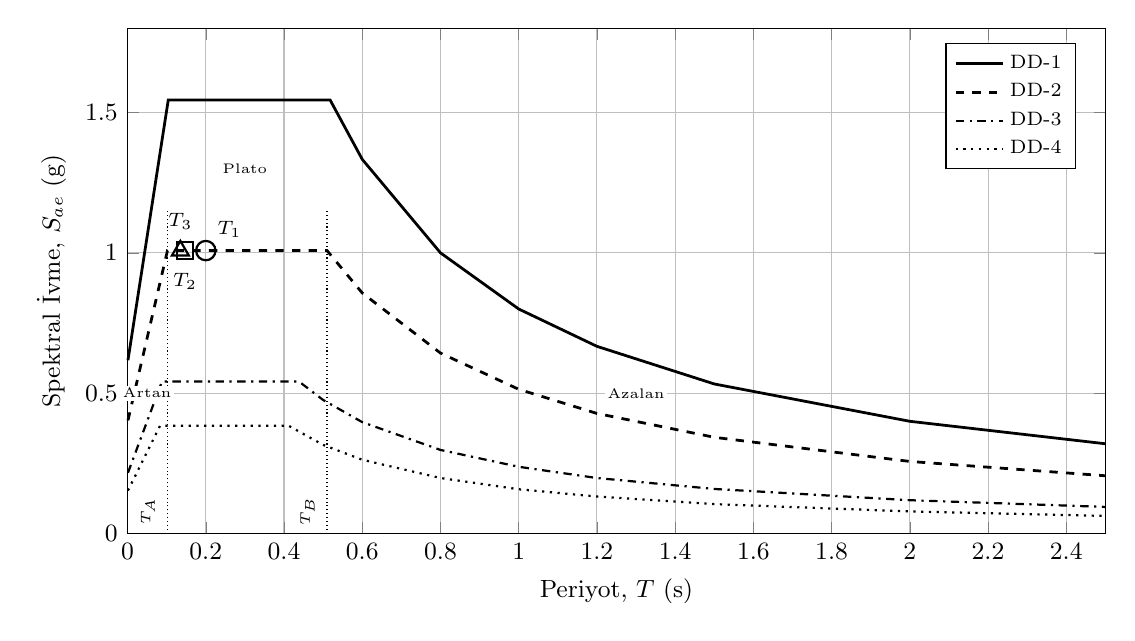
\begin{tikzpicture}
\begin{axis}[
    width=14cm,
    height=8cm,
    xlabel={Periyot, $T$ (s)},
    ylabel={Spektral İvme, $S_{ae}$ (g)},
    xmin=0, xmax=2.5,
    ymin=0, ymax=1.8,
    grid=both,
    grid style={line width=0.2pt, draw=gray!30},
    major grid style={line width=0.4pt, draw=gray!50},
    legend pos=north east,
    legend style={font=\scriptsize, draw=black, fill=white, cells={anchor=west}},
    tick label style={font=\small},
    label style={font=\small},
    every axis plot/.append style={line width=0.8pt},
    clip=false
]

% DD-1 Spektrumu
\addplot[black, solid, line width=1.0pt] coordinates {
    (0.001, 0.6176) (0.104, 1.544) (0.518, 1.544) (0.6, 1.333) (0.8, 1.0) (1.0, 0.8) (1.2, 0.667) (1.5, 0.533) (2.0, 0.4) (2.5, 0.32)
};

% DD-2 Spektrumu
\addplot[black, dashed, line width=1.0pt] coordinates {
    (0.001, 0.4032) (0.102, 1.008) (0.510, 1.008) (0.6, 0.857) (0.8, 0.643) (1.0, 0.514) (1.2, 0.428) (1.5, 0.343) (2.0, 0.257) (2.5, 0.206)
};

% DD-3 Spektrumu
\addplot[black, dashdotted, line width=0.8pt] coordinates {
    (0.001, 0.2168) (0.088, 0.542) (0.438, 0.542) (0.5, 0.476) (0.6, 0.397) (0.8, 0.298) (1.0, 0.238) (1.2, 0.198) (1.5, 0.159) (2.0, 0.119) (2.5, 0.095)
};

% DD-4 Spektrumu
\addplot[black, dotted, line width=0.8pt] coordinates {
    (0.001, 0.1536) (0.083, 0.384) (0.412, 0.384) (0.5, 0.316) (0.6, 0.263) (0.8, 0.198) (1.0, 0.158) (1.2, 0.132) (1.5, 0.105) (2.0, 0.079) (2.5, 0.063)
};

% Modal Analiz - Mod 1
\addplot[only marks, mark=o, mark size=3.5pt, fill=white, draw=black, line width=0.8pt] coordinates {(0.200, 1.008)};
\node[anchor=south west, font=\scriptsize] at (axis cs:0.205, 1.020) {$T_1$};

% Mod 2
\addplot[only marks, mark=square, mark size=3pt, fill=white, draw=black, line width=0.8pt] coordinates {(0.147, 1.008)};
\node[anchor=south, font=\scriptsize] at (axis cs:0.147, 0.835) {$T_2$};

% Mod 3
\addplot[only marks, mark=triangle, mark size=3.5pt, fill=white, draw=black, line width=0.8pt] coordinates {(0.135, 1.008)};
\node[anchor=south, font=\scriptsize] at (axis cs:0.135, 1.050) {$T_3$};

% Köşe periyotları
\addplot[black, thin, densely dotted] coordinates {(0.102, 0) (0.102, 1.15)};
\node[anchor=south, font=\tiny, rotate=90] at (axis cs:0.095, 0.08) {$T_A$};

\addplot[black, thin, densely dotted] coordinates {(0.510, 0) (0.510, 1.15)};
\node[anchor=south, font=\tiny, rotate=90] at (axis cs:0.503, 0.08) {$T_B$};

% Bölge etiketleri
\node[anchor=center, font=\tiny, fill=white, inner sep=1pt] at (axis cs:0.05, 0.50) {Artan};
\node[anchor=center, font=\tiny, fill=white, inner sep=1pt] at (axis cs:0.30, 1.30) {Plato};
\node[anchor=center, font=\tiny, fill=white, inner sep=1pt] at (axis cs:1.3, 0.5) {Azalan};

\legend{DD-1, DD-2, DD-3, DD-4}

\end{axis}
\end{tikzpicture}%
}
\caption{AFAD DD-1/2/3/4 yatay elastik tasarım spektrumları ve \textsc{OpenSees} modal analiz sonuçları (İFM, ZD). Beyaz işaretçiler V9 modelinin ilk üç modunu göstermektedir ($T_1 = 0.200$~s, $T_2 = 0.147$~s, $T_3 = 0.135$~s).}
\label{fig:spectrum}
\end{figure}



\newpage

% ==============================================================================
% SORU 3 (Placeholder)
% ==============================================================================
\subsection{Soru \RN{3}}

\textbf{Soru:} Yapıdaki düşey taşıyıcıların yerleşiminin belirlenmesinde dikkat edilen hususlar nelerdir?

\textbf{Cevap:} Düşey taşıyıcı yerleşiminde üç temel hedef gözetilmiştir: (i)~düşey yüklerin ($Z$) sürekli ve kesintisiz temele aktarımı, (ii)~yatay kuvvetlere ($X$, $Y$) karşı yeterli yanal rijitliğin temini, (iii)~burulma düzensizliğinin kontrolü~\cite{tbdy2018}.

\textit{Kolon Grid Konfigürasyonu:} Her kule için $8 \times 4$ ortogonal kolon gridi uygulanmıştır. $X$ ekseninde değişken açıklık düzeni benimsenmiş olup köşe açıklıkları ($L = 3$~cm) kısa tutularak moment çerçevesi rijitliği artırılmış, merkez bölgede dar kolon aralığı ($\Delta x = 1.2$~cm) ile perde duvarı benzeri rijitlik konsantrasyonu sağlanmıştır. $Y$ ekseninde iç kolon sıraları ($y = 7.4$ ve $8.6$~cm) yakınlaştırılarak köprü bağlantı hattı güçlendirilmiş; bu konfigürasyon rijitlik merkezi ile kütle merkezi arasındaki mesafeyi minimize ederek burulma talebini azaltmaktadır~\cite{nehrp2009}.

\textit{Yanal Yük Taşıyıcı Sistem:} Moment çerçevesi tek başına hedef yanal rijitliği karşılayamadığından, $XZ$ ve $YZ$ düzlemlerinde çapraz elemanlarla desteklenmiş hibrit sistem tercih edilmiştir. Çapraz elemanlar köşe ve merkez açıklıklara yerleştirilmiş; tüm katlarda kesintisiz devam ettirilerek yük akışı sürekliliği tesis edilmiştir~\cite{tbdy2018}.

\textit{Köprü Bağlantı Seviyeleri:} Köprüler yapı yüksekliğinin $H/4$, $H/2$, $3H/4$ ve tepe kotlarına konumlandırılmıştır. Bu dağılım, ikiz kule sistemlerinde mod şekillerini dengeleyerek taban kesme kuvvetini minimize etmektedir~\cite{patoliya2023}. Köprü genişliği merkez kolon hattı ($x = 11$--$19$~cm) ile sınırlandırılmış; böylece kulelerin bağımsız titreşim karakteristiği korunarak kontrollü yük paylaşımı sağlanmıştır. Uygulanan yerleşim düzeni sonucunda kütle-rijitlik eksantrisitesi $e_x/L_x = 0.005$, $e_y/L_y = 0.034$ olarak elde edilmiş; TBDY 2018 sınır değeri ($e/L < 0.05$) sağlanmıştır~\cite{tbdy2018}. Zemin katta A1a burulma düzensizliği katsayısı $\eta_{bi} = 1.25 \gtrapprox 1.2$ olup bu durum temel-üstyapı rijitlik geçişinden kaynaklanmaktadır; üst katlarda $\eta_{bi} < 1.1$ değerleri elde edilmiştir~\cite{teblig2024}. Kolon yerleşimi Şekil~\ref{fig:plan}'de sunulmaktadır.

% ==============================================================================
% ŞEKİL: Kolon Yerleşimi ve Köprü Bağlantısı (Kesit + Plan)
% ==============================================================================
\begin{figure}[H]
\centering
\resizebox{0.95\textwidth}{!}{%
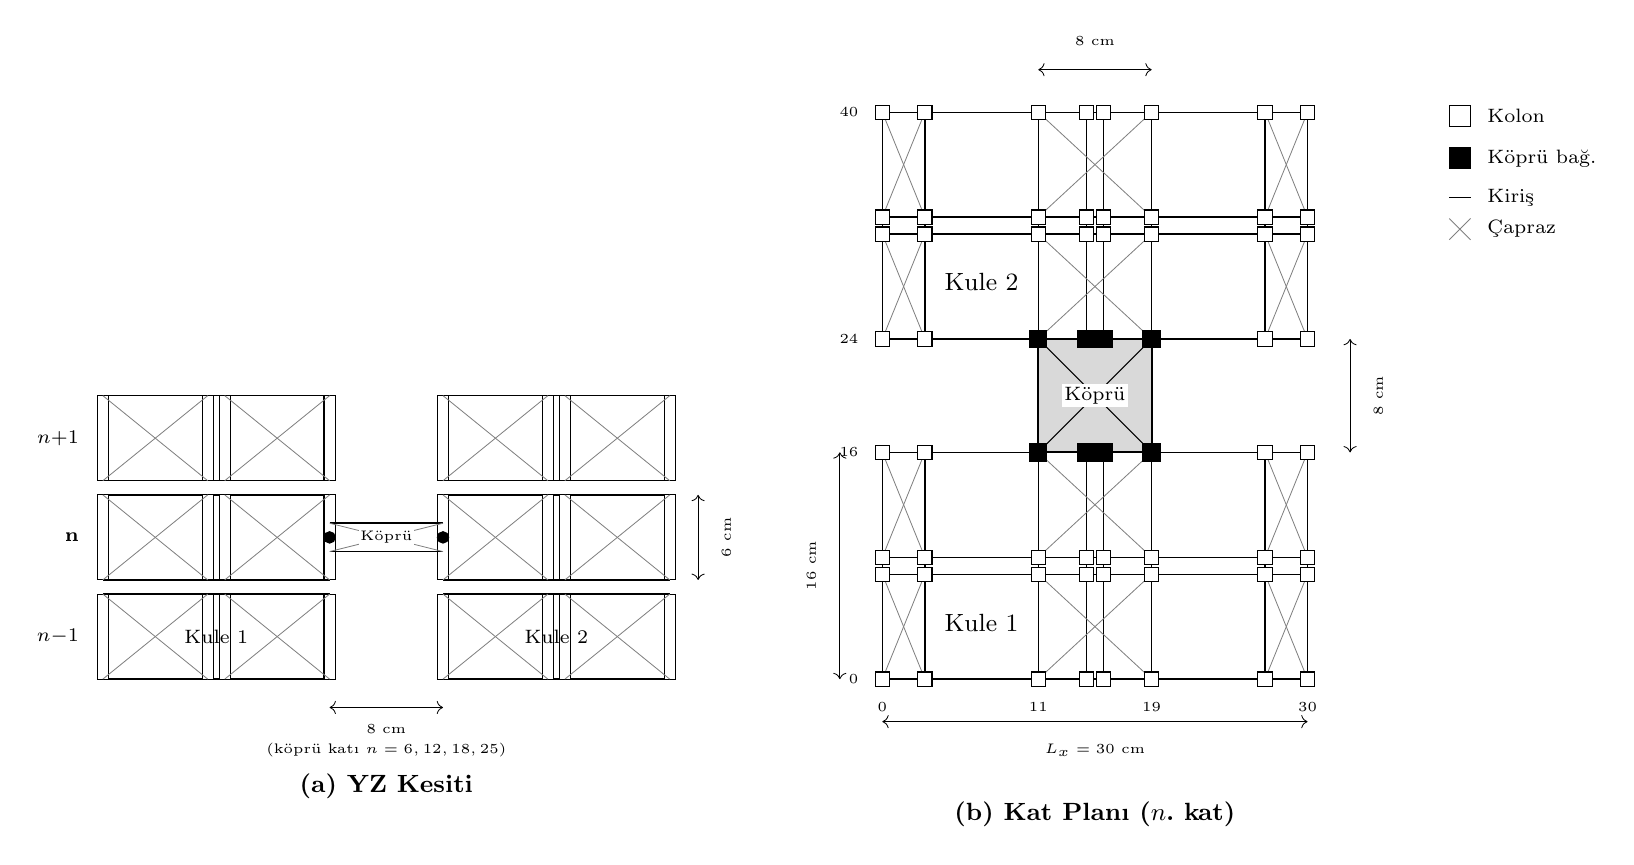
\begin{tikzpicture}[scale=0.18]

% ============== SOL: KESİT GÖRÜNÜMÜ (YZ düzlemi, x=15 kesiti) ==============
\begin{scope}[shift={(0,0)}]
% Kat yüksekliği
\def\kh{6}

% n-1. kat - köprü yok
% Kirişler (üst ve alt)
\draw[line width=0.5pt] (0,0) -- (16,0);
\draw[line width=0.5pt] (24,0) -- (40,0);
\draw[line width=0.5pt] (0,\kh) -- (16,\kh);
\draw[line width=0.5pt] (24,\kh) -- (40,\kh);
% Kolonlar
\foreach \y in {0,7.4,8.6,16,24,31.4,32.6,40} {
    \draw[fill=white, draw=black, line width=0.4pt] (\y-0.4,0) rectangle (\y+0.4,\kh);
}
% X-brace çaprazlar
\draw[line width=0.3pt, gray] (0,0) -- (7.4,\kh);
\draw[line width=0.3pt, gray] (7.4,0) -- (0,\kh);
\draw[line width=0.3pt, gray] (8.6,0) -- (16,\kh);
\draw[line width=0.3pt, gray] (16,0) -- (8.6,\kh);
\draw[line width=0.3pt, gray] (24,0) -- (31.4,\kh);
\draw[line width=0.3pt, gray] (31.4,0) -- (24,\kh);
\draw[line width=0.3pt, gray] (32.6,0) -- (40,\kh);
\draw[line width=0.3pt, gray] (40,0) -- (32.6,\kh);
\node[font=\scriptsize] at (8,\kh/2) {Kule 1};
\node[font=\scriptsize] at (32,\kh/2) {Kule 2};
\node[font=\scriptsize, anchor=east] at (-1,\kh/2) {$n{-}1$};

% n. kat - KÖPRÜ VAR
\begin{scope}[shift={(0,\kh+1)}]
% Kirişler
\draw[line width=0.5pt] (0,0) -- (16,0);
\draw[line width=0.5pt] (24,0) -- (40,0);
\draw[line width=0.5pt] (0,\kh) -- (16,\kh);
\draw[line width=0.5pt] (24,\kh) -- (40,\kh);
% Kolonlar
\foreach \y in {0,7.4,8.6,16,24,31.4,32.6,40} {
    \draw[fill=white, draw=black, line width=0.4pt] (\y-0.4,0) rectangle (\y+0.4,\kh);
}
% X-brace çaprazlar
\draw[line width=0.3pt, gray] (0,0) -- (7.4,\kh);
\draw[line width=0.3pt, gray] (7.4,0) -- (0,\kh);
\draw[line width=0.3pt, gray] (8.6,0) -- (16,\kh);
\draw[line width=0.3pt, gray] (16,0) -- (8.6,\kh);
\draw[line width=0.3pt, gray] (24,0) -- (31.4,\kh);
\draw[line width=0.3pt, gray] (31.4,0) -- (24,\kh);
\draw[line width=0.3pt, gray] (32.6,0) -- (40,\kh);
\draw[line width=0.3pt, gray] (40,0) -- (32.6,\kh);
% KÖPRÜ (y=16 ile y=24 arası, 8cm açıklık)
\draw[line width=0.6pt] (16,2) -- (24,2);
\draw[line width=0.6pt] (16,4) -- (24,4);
\draw[line width=0.3pt, gray] (16,2) -- (24,4);
\draw[line width=0.3pt, gray] (24,2) -- (16,4);
\node[font=\tiny, fill=white, inner sep=0.5pt] at (20,3) {Köprü};
\node[font=\scriptsize, anchor=east] at (-1,\kh/2) {\textbf{n}};
% Köprü bağlantı noktaları
\draw[fill=black] (16,3) circle (0.4);
\draw[fill=black] (24,3) circle (0.4);
\end{scope}

% n+1. kat - köprü yok
\begin{scope}[shift={(0,2*\kh+2)}]
% Kirişler
\draw[line width=0.5pt] (0,0) -- (16,0);
\draw[line width=0.5pt] (24,0) -- (40,0);
\draw[line width=0.5pt] (0,\kh) -- (16,\kh);
\draw[line width=0.5pt] (24,\kh) -- (40,\kh);
% Kolonlar
\foreach \y in {0,7.4,8.6,16,24,31.4,32.6,40} {
    \draw[fill=white, draw=black, line width=0.4pt] (\y-0.4,0) rectangle (\y+0.4,\kh);
}
% X-brace çaprazlar
\draw[line width=0.3pt, gray] (0,0) -- (7.4,\kh);
\draw[line width=0.3pt, gray] (7.4,0) -- (0,\kh);
\draw[line width=0.3pt, gray] (8.6,0) -- (16,\kh);
\draw[line width=0.3pt, gray] (16,0) -- (8.6,\kh);
\draw[line width=0.3pt, gray] (24,0) -- (31.4,\kh);
\draw[line width=0.3pt, gray] (31.4,0) -- (24,\kh);
\draw[line width=0.3pt, gray] (32.6,0) -- (40,\kh);
\draw[line width=0.3pt, gray] (40,0) -- (32.6,\kh);
\node[font=\scriptsize, anchor=east] at (-1,\kh/2) {$n{+}1$};
\end{scope}

% Boyutlar
\draw[<->, line width=0.3pt] (16,-2) -- (24,-2);
\node[font=\tiny] at (20,-3.5) {8 cm};
\draw[<->, line width=0.3pt] (42,\kh+1) -- (42,\kh+1+\kh);
\node[font=\tiny, rotate=90] at (44,\kh+4) {6 cm};

\node[font=\small, anchor=north] at (20,-6) {\textbf{(a) YZ Kesiti}};
\node[font=\tiny] at (20,-5) {(köprü katı $n = 6, 12, 18, 25$)};
\end{scope}

% ============== SAĞ: PLAN GÖRÜNÜMÜ (n. kat) ==============
\begin{scope}[shift={(55,0)}]

% Kirişler X yönü (Kule 1)
\foreach \y in {0,7.4,8.6,16} {
    \draw[line width=0.5pt] (0,\y) -- (30,\y);
}
% Kirişler X yönü (Kule 2)
\foreach \y in {24,31.4,32.6,40} {
    \draw[line width=0.5pt] (0,\y) -- (30,\y);
}
% Kirişler Y yönü (Kule 1)
\foreach \x in {0,3,11,14.4,15.6,19,27,30} {
    \draw[line width=0.5pt] (\x,0) -- (\x,16);
}
% Kirişler Y yönü (Kule 2)
\foreach \x in {0,3,11,14.4,15.6,19,27,30} {
    \draw[line width=0.5pt] (\x,24) -- (\x,40);
}

% X-Brace döşeme (Kule 1) - her panelde çapraz
\draw[line width=0.3pt, gray] (0,0) -- (3,7.4);
\draw[line width=0.3pt, gray] (3,0) -- (0,7.4);
\draw[line width=0.3pt, gray] (27,0) -- (30,7.4);
\draw[line width=0.3pt, gray] (30,0) -- (27,7.4);
\draw[line width=0.3pt, gray] (0,8.6) -- (3,16);
\draw[line width=0.3pt, gray] (3,8.6) -- (0,16);
\draw[line width=0.3pt, gray] (27,8.6) -- (30,16);
\draw[line width=0.3pt, gray] (30,8.6) -- (27,16);
% Merkez X-brace
\draw[line width=0.3pt, gray] (11,0) -- (19,7.4);
\draw[line width=0.3pt, gray] (19,0) -- (11,7.4);
\draw[line width=0.3pt, gray] (11,8.6) -- (19,16);
\draw[line width=0.3pt, gray] (19,8.6) -- (11,16);

% X-Brace döşeme (Kule 2)
\draw[line width=0.3pt, gray] (0,24) -- (3,31.4);
\draw[line width=0.3pt, gray] (3,24) -- (0,31.4);
\draw[line width=0.3pt, gray] (27,24) -- (30,31.4);
\draw[line width=0.3pt, gray] (30,24) -- (27,31.4);
\draw[line width=0.3pt, gray] (0,32.6) -- (3,40);
\draw[line width=0.3pt, gray] (3,32.6) -- (0,40);
\draw[line width=0.3pt, gray] (27,32.6) -- (30,40);
\draw[line width=0.3pt, gray] (30,32.6) -- (27,40);
% Merkez X-brace
\draw[line width=0.3pt, gray] (11,24) -- (19,31.4);
\draw[line width=0.3pt, gray] (19,24) -- (11,31.4);
\draw[line width=0.3pt, gray] (11,32.6) -- (19,40);
\draw[line width=0.3pt, gray] (19,32.6) -- (11,40);

% Kule 1 kolonları
\foreach \x in {0,3,11,14.4,15.6,19,27,30} {
    \foreach \y in {0,7.4,8.6,16} {
        \draw[fill=white, draw=black, line width=0.4pt] (\x-0.5,\y-0.5) rectangle (\x+0.5,\y+0.5);
    }
}
% Kule 2 kolonları
\foreach \x in {0,3,11,14.4,15.6,19,27,30} {
    \foreach \y in {24,31.4,32.6,40} {
        \draw[fill=white, draw=black, line width=0.4pt] (\x-0.5,\y-0.5) rectangle (\x+0.5,\y+0.5);
    }
}

% KÖPRÜ - sadece x=11 ile x=19 arası (8cm), y=16 ile y=24 arası (8cm)
\draw[fill=gray!30, draw=black, line width=0.8pt] (11,16) rectangle (19,24);
% Köprü X-brace
\draw[line width=0.4pt] (11,16) -- (19,24);
\draw[line width=0.4pt] (19,16) -- (11,24);
\node[font=\scriptsize, fill=white, inner sep=1pt] at (15,20) {Köprü};

% Köprü bağlantı kolonları (vurgulu)
\foreach \x in {11,14.4,15.6,19} {
    \draw[fill=black, draw=black, line width=0.5pt] (\x-0.6,16-0.6) rectangle (\x+0.6,16+0.6);
    \draw[fill=black, draw=black, line width=0.5pt] (\x-0.6,24-0.6) rectangle (\x+0.6,24+0.6);
}

% Etiketler
\node[font=\small] at (7,4) {Kule 1};
\node[font=\small] at (7,28) {Kule 2};

% Boyutlar
\draw[<->, line width=0.3pt] (0,-3) -- (30,-3);
\node[font=\tiny] at (15,-5) {$L_x = 30$ cm};
\draw[<->, line width=0.3pt] (-3,0) -- (-3,16);
\node[font=\tiny, rotate=90] at (-5,8) {16 cm};
\draw[<->, line width=0.3pt] (33,16) -- (33,24);
\node[font=\tiny, rotate=90] at (35,20) {8 cm};
\draw[<->, line width=0.3pt] (11,43) -- (19,43);
\node[font=\tiny] at (15,45) {8 cm};

% Koordinatlar
\node[font=\tiny, anchor=north] at (0,-1) {0};
\node[font=\tiny, anchor=north] at (11,-1) {11};
\node[font=\tiny, anchor=north] at (19,-1) {19};
\node[font=\tiny, anchor=north] at (30,-1) {30};
\node[font=\tiny, anchor=east] at (-1,0) {0};
\node[font=\tiny, anchor=east] at (-1,16) {16};
\node[font=\tiny, anchor=east] at (-1,24) {24};
\node[font=\tiny, anchor=east] at (-1,40) {40};

\node[font=\small, anchor=north] at (15,-8) {\textbf{(b) Kat Planı ($n$. kat)}};
\end{scope}

% ============== LEGEND ==============
\begin{scope}[shift={(95,25)}]
\draw[fill=white, draw=black, line width=0.4pt] (0,14) rectangle (1.5,15.5);
\node[font=\scriptsize, anchor=west] at (2,14.75) {Kolon};
\draw[fill=black, draw=black, line width=0.4pt] (0,11) rectangle (1.5,12.5);
\node[font=\scriptsize, anchor=west] at (2,11.75) {Köprü bağ.};
\draw[line width=0.5pt] (0,9) -- (1.5,9);
\node[font=\scriptsize, anchor=west] at (2,9) {Kiriş};
\draw[line width=0.3pt, gray] (0,6) -- (1.5,7.5);
\draw[line width=0.3pt, gray] (1.5,6) -- (0,7.5);
\node[font=\scriptsize, anchor=west] at (2,6.75) {Çapraz};
\end{scope}

\end{tikzpicture}%
}
\caption{V9 modeli kolon yerleşimi ve köprü bağlantısı: (a)~YZ kesiti ($n{-}1$, $n$, $n{+}1$ katları), (b)~köprü katı planı. Şekil temsili ve ölçeklendirilmemiştir. Temsilî çizim için DASK 2026 kodları~\cite{github_repo} kullanılmıştır.}
\label{fig:plan}
\end{figure}

\newpage

% ==============================================================================
% SORU 4
% ==============================================================================
\subsection{Soru \RN{4}}

\textbf{Soru:} Önerdiğiniz yapısal sistemin ülkemizde uygulaması yaygın mıdır? Yaygın değilse sebepleri ne olabilir? Bu sebepler arasında uygulama zorluğu ve maliyet olabilir mi?

\textbf{Cevap:} Önerilen ikiz kule--gökyüzü köprüsü--moment çerçevesi/çaprazlı çerçeve hibrit sistemi Türkiye'de \textbf{yaygın değildir}. Ülkemiz dünyanın 7.~büyük ham çelik üreticisi olmasına karşın yapısal çeliğin inşaat sektöründeki payı \%5'in altındadır; gelişmiş ülkelerde bu oran \%30--55 bandındadır~\cite{kurtay2004, of2022}. İkiz kule konsepti yalnızca İş Kuleleri, Tat Towers ve Skyland İstanbul gibi sınırlı sayıda projede karşımıza çıkmakta; hiçbirinde yüksek kotta kuleleri bağlayan yapısal bir sky bridge bulunmamaktadır. Petronas İkiz Kuleleri (170~m kotunda 58~m çelik köprü) bu konfigürasyonun dünya ölçeğindeki en bilinen temsilcisi olup Türkiye'de eşdeğeri mevcut değildir~\cite{patoliya2023}.

\subsubsection{Uygulama Zorluğu}

Hibrit sistemde moment çerçevesi düğüm noktaları tam nüfuziyetli küt kaynak ile rijit bağlantı gerektirmekte; her birleşimin ultrasonik muayene (UT) ile tahribatsız kontrol sürecinden geçmesi zorunludur. Çaprazlı çerçevelerde ise guse plakası tasarımı Whitmore efektif kesit, blok kesme dayanımı ve burkulma kontrolleri gibi çok parametreli bir detaylandırma sürecini içermektedir. Sky bridge elemanları, iki bağımsız kulenin farklı titreşim periyotlarından kaynaklanan diferansiyel yer değiştirmelere maruz kaldığından kayma anahtarı, sismik derz veya sürgülü mesnet gibi özel birleşim detayları ile donatılmalıdır. Türkiye'de çelik yapı sektörü betonarmeye kıyasla oldukça dar kapsamlıdır; sertifikalı kaynak teknisyeni, çelik detay mühendisi ve bu tür karmaşık birleşimleri projelendirebilecek deneyimli yapısal tasarım bürosu sayısı sınırlı kalmaktadır~\cite{kurtay2004}.

\subsubsection{Maliyet}

Çelik malzemenin kilogram başına birim fiyatı betonarmeye yakın olmakla birlikte sistemin bütünü değerlendirildiğinde belirgin ek maliyet kalemleri ortaya çıkmaktadır: tam nüfuziyetli kaynak işçiliği, UT ve manyetik parçacık muayenesi (MT) gibi tahribatsız muayene süreçleri, epoksi veya galvaniz bazlı çok katmanlı korozyon koruma sistemi ve sky bridge özel çelik imalatı bunların başlıcalarıdır. Öte yandan çeliğin düşük özgül ağırlığı ($\gamma_s \approx 78.5$~kN/m\textsuperscript{3}$\ll \gamma_c \approx 25$~kN/m\textsuperscript{3}) yapının toplam kütlesini $m_t$ ciddi oranda azaltmakta, taban kesme kuvveti $V_{tE}=m_t\,S_{aR}(T_1)$ doğrudan düşmekte ve temel boyutları küçülmektedir~\cite{tbdy2018}. Ayrıca fabrikada kontrollü üretim ile sahada bulonlu montaj, kalıp-iskele ihtiyacını ortadan kaldırarak inşaat süresini ve işçilik maliyetini belirgin biçimde azaltmaktadır.

\subsubsection{Sektörel Sebepler}

Türkiye'de inşaat sektörü köklü bir betonarme geleneği üzerine inşa edilmiştir. Ülke genelinde çimento fabrikası, hazır beton santrali ve beton prefabrik tesisi altyapısı son derece güçlüdür; mühendislik fakültelerinde yapısal tasarım eğitimi ağırlıklı olarak betonarme üzerine şekillenmektedir. Çelik yapıların tasarım, hesap ve yapım esaslarını düzenleyen ulusal yönetmelik ÇYTHYE 2018 ancak son yıllarda yürürlüğe girmiş olup~\cite{cythye2018} sektörde çelik yapı kültürünün oluşması için yeterli süre henüz geçmemiştir. Deprem sonrası hızlı yeniden yapılanma ihtiyacı ve çeliğin sismik performans avantajları göz önüne alındığında~\cite{of2022} bu eğilimin değişeceği ve önerdiğimiz gibi hibrit sistemlerin ülkemizde giderek daha fazla tatbik edileceği öngörülmektedir.

\newpage

% ==============================================================================
% SORU 5 (Placeholder)
% ==============================================================================
\subsection{Soru \RN{5}}

\textbf{Soru:} Deprem etkileri altında tasarıma esas iç kuvvetleri belirlemek için hangi hesap yöntemini seçtiğinizi nedenleriyle birlikte açıklayınız.

\textbf{Cevap:} Tasarıma esas iç kuvvetlerin tayininde \textbf{Mod Birleştirme Yöntemi} (MBY, TBDY 2018 Md.~4.8.2) tercih edilmiştir~\cite{tbdy2018}.

\subsubsection{EDYY'nin Yetersizliği}

Eşdeğer Deprem Yükü Yöntemi (EDYY, Md.~4.7.3) yapı davranışının birinci mod ile temsil edilebileceğini varsayar. Kat deprem kuvvetleri bu tek modun şekil fonksiyonuna istinaden dağıtılır. Ne var ki ikiz kule--köprü sisteminde köprü elemanları iki kulenin müstakil titreşim modlarını çiftleştirmekte; translasyonel ve torsiyonel bileşenleri müteselsilen ihtiva eden karışık modlar hasıl olmaktadır. İlk üç doğal periyot ($T_1=0.200$~s, $T_2=0.147$~s, $T_3=0.135$~s) birbirine yakındır; birinci modun etkin kütle oranı yalnızca \%42'dir. Kalan katkı üst modlara tevzi olmaktadır. Bu husus EDYY'nin esas varsayımını geçersiz kılmaktadır~\cite{tbdy2018}.

\subsubsection{MBY'nin Tercih Gerekçesi}

MBY'de tüm anlamlı titreşim modları ayrı ayrı göz önüne alınır. Her $n$.~mod için azaltılmış spektral ivme $S_{aR}(T_n) = S_{ae}(T_n)/R_a(T_n)$ tasarım spektrumundan okunur; modal kütle ile çarpılarak ilgili moda ait deprem kuvveti elde edilir ($R=4$, $D=2.5$, $I=1.0$). Elde edilen modal kuvvetler elemanlarda $N$, $V$, $M$ iç tesirlerine dönüştürülüp istatistiksel bir kaide ile tevhid edilir. İlk üç modun yakın frekansları hasebiyle modlar arası korelasyon ihmal edilemez; bu sebeple SRSS yerine \textbf{CQC} kuralı ($\xi=0.05$) benimsenmiştir. Denk.~4.30 muktezasınca her iki doğrultuda etkin kütle oranı toplamı \%95'i aşıncaya dek mod sayısı artırılmış; 12 mod ile şart sağlanmıştır~\cite{tbdy2018}.

Taban kesme kuvveti Md.~4.8.4 Denk.~4.31 uyarınca $\beta_{tE}$ ile kontrol edilmiş; A1a düzensizliği sebebiyle $\gamma_E = 0.90$ alınmıştır. Göreli kat ötelemesinde çelik yapılara mahsus $\kappa = 0.5$ (Md.~4.9.1.4) gözetilmiş; ikinci mertebe etkileri $C_h = 1$ ile hesaba katılmıştır (Md.~4.9.2)~\cite{tbdy2018, cythye2018}.

\subsubsection{Doğrulama ve Ölçekli Model}

\textsc{OpenSees}\textsuperscript{\textregistered}~\cite{opensees} ile 1680 düğüm, 4248 \texttt{elasticBeamColumn} elemanlı V9 modeli tesis edilmiştir. MBY neticeleri iki müstakil yöntemle teyit edilmiştir: ZTAH (Md.~4.8.3; Düzce BOL090, $1/\!\sqrt{50}$ ölçek, Newmark-$\beta$, $\Delta t = 0.005$~s) ve statik itme (Md.~5.6.5; ters üçgen yük, $\delta_t = 6.12$~cm)~\cite{github_repo}. Her iki tahlilde taban kesme kuvveti ve kat ötelemesi MBY ile mutabık bulunmuştur.

TBDY 2018 usulleri gerçek ölçekli binalar için tanzim edilmiş olmakla birlikte dayandığı nazari esaslar ölçekten bağımsızdır. Özdeğer problemi, CQC ve modal süperpozisyon sırf riyazi işlemlerdir; yapının balsa ($E\!=\!3.5$~GPa) yahut çelik ($E\!=\!200$~GPa) olması yalnızca $\mathbf{K}$ ve $\mathbf{M}$'yi değiştirir. Benzeşim kuramı gereğince $S_F\!=\!S_E S_L^2$, $S_m\!=\!S_\rho S_L^3$ şartı sağlandıkça bu yöntemler ölçekli modelde de mer'iyyetini muhafaza etmektedir~\cite{tbdy2018}.

\newpage

% ==============================================================================
% SORU 6 (Placeholder)
% ==============================================================================
\subsection{Soru \RN{6}}

\textbf{Soru:} Yapı analizinde sönüm oranının ne şekilde dikkate alındığını açıklayınız.

\textbf{Cevap:} Sönüm, deprem enerjisinin yapı içinde yutulmasını temsil eden ve dinamik tepkiyi doğrudan tayin eden parametredir. Analizlerde (i)~tasarım spektrumunda sönüm düzeltmesi, (ii)~ZTAH'de Rayleigh sönümü olmak üzere iki seviyede dikkate alınmıştır~\cite{tbdy2018}.

\subsubsection{Tasarım Spektrumu ve Sönüm Düzeltmesi}

TBDY 2018 elastik tasarım spektrumu $\xi = \%5$ esas alınarak tanzim edilmiştir. Farklı sönüm nispetinde spektral ordinatlar $\eta_b = \sqrt{10/(5 + \xi\,(\%))}$ katsayısı ile tashih edilir (Md.~2.3.4): $\xi = \%2$ için $\eta_b = 1.195$; $\xi = \%5$ için $\eta_b = 1.00$; $\xi = \%10$ için $\eta_b = 0.816$~\cite{tbdy2018}. Modelimizde $\xi = \%5$ kabul edilmiştir; bu değer çelik çerçeve yapılar ($\%2$--$\%5$) ile uyumludur~\cite{cythye2018}.

\subsubsection{Rayleigh Sönümü}

ZTAH'de hareket denklemi $\mathbf{M}\ddot{\mathbf{u}} + \mathbf{C}\dot{\mathbf{u}} + \mathbf{K}\mathbf{u} = -\mathbf{M}\mathbf{1}\ddot{u}_g(t)$ olup sönüm matrisi Rayleigh formülasyonuyla $\mathbf{C} = a_0\mathbf{M} + a_1\mathbf{K}$ şeklinde tesis edilir. Herhangi $n$.~modun sönüm oranı $\xi_n = a_0/(2\omega_n) + a_1\omega_n/2$'dir. İki kontrol frekansında hedef $\xi$ sağlanacak biçimde $a_0 = 2\xi\omega_i\omega_j/(\omega_i+\omega_j)$, $a_1 = 2\xi/(\omega_i+\omega_j)$ hesaplanır~\cite{opensees}.

V9 modelinde $\omega_1 = 2\pi/T_1 = 31.43$~rad/s ve $\omega_2 = 3.5\omega_1 = 110.0$~rad/s seçilmiş; $\xi = 0.05$ ile $a_0 = 2.443$, $a_1 = 7.07 \times 10^{-4}$~s elde edilmiştir. Bu iki frekans arasında sönüm oranı hedefin altında kalır ($\xi_{min} = 0.0416$); yüksek modlarda aşırı sönüm hasıl olarak sahte salınımlar bastırılır. \textsc{OpenSees}\textsuperscript{\textregistered}'de \texttt{rayleigh \$a0 \$a1 0 0} komutuyla atanmıştır; elastik modelde $\mathbf{K}_0 = \mathbf{K}_t$ olduğundan son iki argüman sıfırdır. Frekansa göre efektif sönüm oranı: $T = 0.050$~s'de $\xi = 0.064$; $T_3 = 0.135$~s'de $\xi = 0.042$; $T_1 = 0.200$~s'de $\xi = 0.050$; $T = 0.500$~s'de $\xi = 0.117$.

\subsubsection{Sönümün Yapı Tepkisine Tesiri}

KYH-1 (PGA $= 0.335$~g) altında $\xi = \%2$ ile çatı ötelemesi $u_{max} = 0.486$~cm elde edilmiş; $\xi = \%5$'te $\eta_b$ düzeltmesi ($\approx 0.84$) ile ${\sim}0.41$~cm mertebesine inmesi beklenir. Sönüm iki katına çıktığında tepki $\%15$--$\%20$ azalmakta, yarıya düştüğünde aynı oranda artmaktadır. MBY'de sönüm etkisi spektrum üzerinden yansır; ZTAH'de Rayleigh formülasyonuyla her moda ayrı ayrı atanır. Her iki yaklaşımda sonuçlar tutarlıdır~\cite{tbdy2018}.

\newpage

% ==============================================================================
% SORU 7 (Placeholder)
% ==============================================================================
\subsection{Soru \RN{7}}


\textit{Bu bölüm daha sonra doldurulacaktır.}

\newpage

% ==============================================================================
% SORU 8 (Placeholder)
% ==============================================================================
\subsection{Soru \RN{8}}


\textit{Bu bölüm daha sonra doldurulacaktır.}

\newpage

% ==============================================================================
% KAYNAKLAR
% ==============================================================================
\begin{thebibliography}{99}

\bibitem{tbdy2018} T.C. Çevre ve Şehircilik Bakanlığı, \textit{Türkiye Bina Deprem Yönetmeliği (TBDY 2018)}, Resmi Gazete, 2018.

\bibitem{teblig2024} T.C. Çevre, Şehircilik ve İklim Değişikliği Bakanlığı, \textit{TBDY 2018 Uygulama Tebliği Taslağı}, 27.05.2024.

\bibitem{afad2024} AFAD, \textit{Türkiye Deprem Tehlike Haritaları İnteraktif Web Uygulaması}, \url{https://tdth.afad.gov.tr}, 2024.

\bibitem{opensees} McKenna, F., Scott, M.H., Fenves, G.L., \textit{OpenSees: Open System for Earthquake Engineering Simulation}, Pacific Earthquake Engineering Research Center, UC Berkeley, \url{https://opensees.berkeley.edu}.
\bibitem{nehrp2009} FEMA P-751, \textit{2009 NEHRP Recommended Seismic Provisions: Design Examples}, Building Seismic Safety Council, National Institute of Building Sciences, Washington, D.C., 2012.

\bibitem{patoliya2023} Patoliya, N., Patel, I., Agrawal, V., Seismic Analysis of Tall Buildings Connected with Sky Bridge, \textit{IARJSET}, vol.~10, 2023, doi: 10.17148/IARJSET.2023.10446.

\bibitem{github_repo} Adzetto, \textit{DASK 2026 Tasarım ve Analiz Kodları}, \url{https://github.com/adzetto/DASK_26__DESIGN_AND_ANALYSIS}, 2026.

\bibitem{cythye2018} T.C. Çevre ve Şehircilik Bakanlığı, \textit{Çelik Yapıların Tasarım, Hesap ve Yapım Esaslarına Dair Yönetmelik (ÇYTHYE 2018)}, Resmi Gazete, 2018.

\bibitem{kurtay2004} Kurtay, C., Badem, M., Avrupa Ülkeleri ve Türkiye'deki Çelik Yapı Uygulama Olanak ve Kısıtlarının İncelenmesi, \textit{Gazi Üniversitesi Mühendislik Mimarlık Fakültesi Dergisi}, cilt~19, sayı~4, ss.~351--363, 2004.

\bibitem{of2022} Of, N., Öztürk, S., Depremlerden Sonraki Yeniden Yapılanma Süreci Üzerine Küresel Bir Araştırma: Çelik Prefabrik Malzeme Kullanımının Gerekliliği, \textit{Afet ve Risk Dergisi}, cilt~5, sayı~1, ss.~346--360, 2022, doi: 10.35341/afet.1092649.

\bibitem{tambunan2024} Tambunan, M.L.S., Sjah, J., Rarasati, A.D., Sulistian, R., Trigunarsyah, B., Optimizing Seismic Design of Multi-Tower Buildings Using Sky Bridge Isolation and BIM: A Case Study, \textit{Int.\ J.\ Eng.\ Technol.\ Innov.}, vol.~14, no.~4, pp.~355--377, 2024, doi: 10.46604/ijeti.2024.13409.

\end{thebibliography}

\end{document}
